\begin{figure}[H]
\providecommand{\sseventeenaxisscale}{linear}
\centering
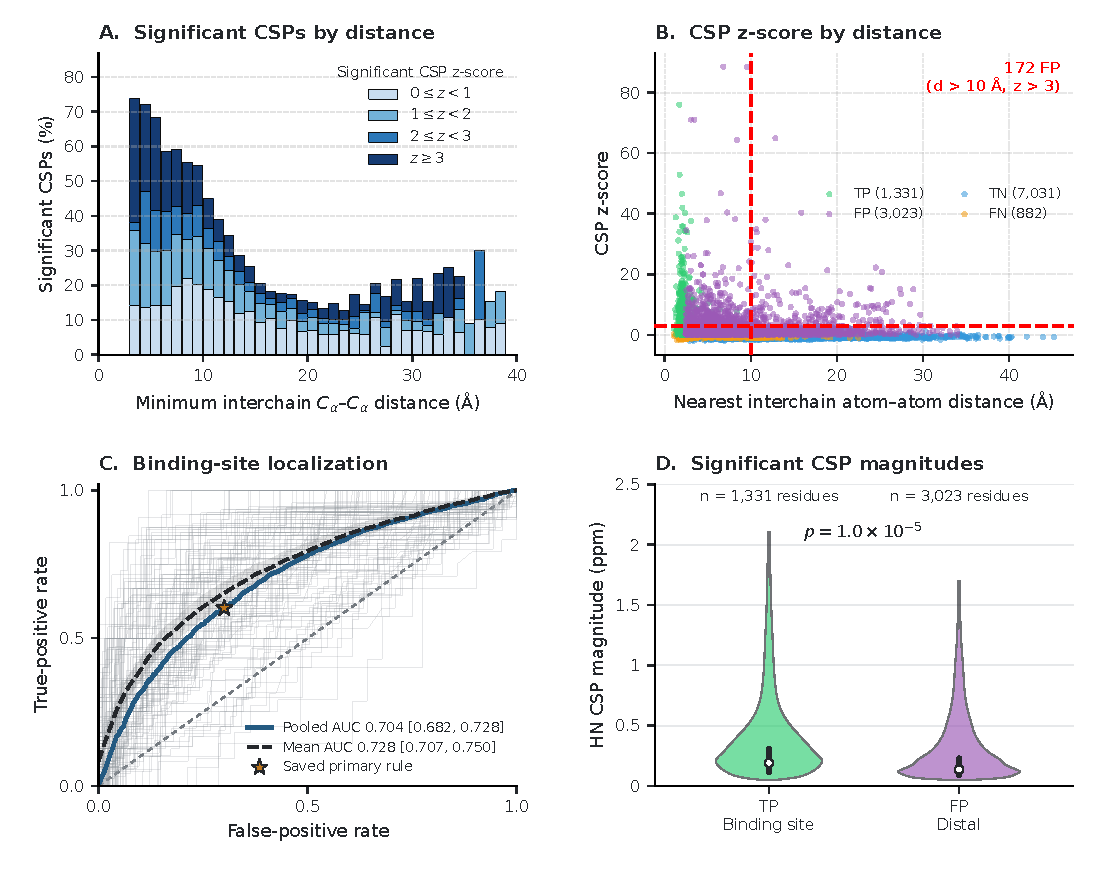
\includegraphics[width=\linewidth]{SF17_csp_distance_and_binding_site.pdf}
\captionsetup{labelformat=empty}
\caption[CSPs and structural binding-site localization]{%
\textbf{SI Fig. S17. CSPs and structural binding-site localization.}
All panels use 135 pH- and temperature-matched apo/holo targets. The per-target
cutoff is $\max(\text{cleaned mean HN CSP},\,0.05\,\mathrm{ppm})$.
\textbf{A.}~Percentage of residues with a significant HN CSP among those with a
recorded CSP in each 1\,\AA{} bin of minimum interchain
$C_\alpha$--$C_\alpha$ distance. Stacks partition the significant fraction by
CSP $z$-score.
\textbf{B.}~Per-residue CSP $z$-score versus nearest interchain atom--atom
distance. For residue $i$, $z_i=(\mathrm{CSP}_i-\mu_{\mathrm{clean}})/\sigma_{\mathrm{clean}}$,
where $\mu_{\mathrm{clean}}$ and $\sigma_{\mathrm{clean}}$ are the mean and population
standard deviation of the target's HN CSP list after iterative removal of high
outliers. Colors indicate true positives (TP), false positives (FP), true
negatives (TN), and false negatives (FN) relative to the structural binding-site
definition. Dashed lines mark $z=3$ and $d=10$\,\AA{}. The 172 annotated FPs
exceed both thresholds.
\textbf{C.}~Receiver operating characteristic (ROC) curves across HN CSP
thresholds for 12,267 eligible residues. Gray curves show individual targets,
blue shows the pooled ROC using CSP divided by the target-specific cutoff, and
the black dashed curve shows the equal-target mean ROC. The pooled area under
the curve (AUC) is 0.704 (95\% CI 0.682--0.728), and the mean per-target AUC is
0.728 (95\% CI 0.707--0.750). The band shows the pointwise 95\% interval for the
mean ROC. Intervals use 2,000 whole-target bootstrap replicates. The gray diagonal
indicates chance, and the star marks the pooled operating point from the saved
primary significance calls.
\textbf{D.}~HN CSP magnitudes for 1,331 significant binding-site residues (TP,
green) and 3,023 significant distal residues (FP, purple) under the saved
primary rule, pooled across targets. Scott-bandwidth kernel densities are
estimated and normalized to equal area in $\log_{10}$ CSP space and bounded by
the observed ranges. White dots mark medians and black bars mark interquartile
ranges. The y-axis is \sseventeenaxisscale{} (ppm). The symmetric
Kullback--Leibler divergence was 0.0941 nats (20 shared log-spaced bins, 0.5 pseudocount per bin),
with $p=1.0\times10^{-5}$ from 99,999 within-target label permutations.}
\end{figure}
